% Options for packages loaded elsewhere
% Options for packages loaded elsewhere
\PassOptionsToPackage{unicode}{hyperref}
\PassOptionsToPackage{hyphens}{url}
%
\documentclass[
  english,
  russian,
  12pt,
  a4paper,
  DIV=11,
  numbers=noendperiod]{scrreprt}
\usepackage{xcolor}
\usepackage{amsmath,amssymb}
\setcounter{secnumdepth}{5}
\usepackage{iftex}
\ifPDFTeX
  \usepackage[T1]{fontenc}
  \usepackage[utf8]{inputenc}
  \usepackage{textcomp} % provide euro and other symbols
\else % if luatex or xetex
  \usepackage{unicode-math} % this also loads fontspec
  \defaultfontfeatures{Scale=MatchLowercase}
  \defaultfontfeatures[\rmfamily]{Ligatures=TeX,Scale=1}
\fi
\usepackage{lmodern}
\ifPDFTeX\else
  % xetex/luatex font selection
\fi
% Use upquote if available, for straight quotes in verbatim environments
\IfFileExists{upquote.sty}{\usepackage{upquote}}{}
\IfFileExists{microtype.sty}{% use microtype if available
  \usepackage[]{microtype}
  \UseMicrotypeSet[protrusion]{basicmath} % disable protrusion for tt fonts
}{}
\usepackage{setspace}
% Make \paragraph and \subparagraph free-standing
\makeatletter
\ifx\paragraph\undefined\else
  \let\oldparagraph\paragraph
  \renewcommand{\paragraph}{
    \@ifstar
      \xxxParagraphStar
      \xxxParagraphNoStar
  }
  \newcommand{\xxxParagraphStar}[1]{\oldparagraph*{#1}\mbox{}}
  \newcommand{\xxxParagraphNoStar}[1]{\oldparagraph{#1}\mbox{}}
\fi
\ifx\subparagraph\undefined\else
  \let\oldsubparagraph\subparagraph
  \renewcommand{\subparagraph}{
    \@ifstar
      \xxxSubParagraphStar
      \xxxSubParagraphNoStar
  }
  \newcommand{\xxxSubParagraphStar}[1]{\oldsubparagraph*{#1}\mbox{}}
  \newcommand{\xxxSubParagraphNoStar}[1]{\oldsubparagraph{#1}\mbox{}}
\fi
\makeatother


\usepackage{longtable,booktabs,array}
\usepackage{calc} % for calculating minipage widths
% Correct order of tables after \paragraph or \subparagraph
\usepackage{etoolbox}
\makeatletter
\patchcmd\longtable{\par}{\if@noskipsec\mbox{}\fi\par}{}{}
\makeatother
% Allow footnotes in longtable head/foot
\IfFileExists{footnotehyper.sty}{\usepackage{footnotehyper}}{\usepackage{footnote}}
\makesavenoteenv{longtable}
\usepackage{graphicx}
\makeatletter
\newsavebox\pandoc@box
\newcommand*\pandocbounded[1]{% scales image to fit in text height/width
  \sbox\pandoc@box{#1}%
  \Gscale@div\@tempa{\textheight}{\dimexpr\ht\pandoc@box+\dp\pandoc@box\relax}%
  \Gscale@div\@tempb{\linewidth}{\wd\pandoc@box}%
  \ifdim\@tempb\p@<\@tempa\p@\let\@tempa\@tempb\fi% select the smaller of both
  \ifdim\@tempa\p@<\p@\scalebox{\@tempa}{\usebox\pandoc@box}%
  \else\usebox{\pandoc@box}%
  \fi%
}
% Set default figure placement to htbp
\def\fps@figure{htbp}
\makeatother



\ifLuaTeX
\usepackage[bidi=basic,provide=*]{babel}
\else
\usepackage[bidi=default,provide=*]{babel}
\fi
% get rid of language-specific shorthands (see #6817):
\let\LanguageShortHands\languageshorthands
\def\languageshorthands#1{}


\setlength{\emergencystretch}{3em} % prevent overfull lines

\providecommand{\tightlist}{%
  \setlength{\itemsep}{0pt}\setlength{\parskip}{0pt}}



 
\usepackage[style=gost-numeric,backend=biber,langhook=extras,autolang=other*]{biblatex}
\addbibresource{bib/cite.bib}

\usepackage[]{csquotes}

\KOMAoption{captions}{tableheading}
\usepackage{indentfirst}
\usepackage{float}
\floatplacement{figure}{H}
\usepackage{libertine}
\usepackage{indentfirst}
\usepackage{float}
\floatplacement{figure}{H}
\usepackage[math,RM={Scale=0.94},SS={Scale=0.94},SScon={Scale=0.94},TT={Scale=MatchLowercase,FakeStretch=0.9},DefaultFeatures={Ligatures=Common}]{plex-otf}
\makeatletter
\@ifpackageloaded{caption}{}{\usepackage{caption}}
\AtBeginDocument{%
\ifdefined\contentsname
  \renewcommand*\contentsname{Содержание}
\else
  \newcommand\contentsname{Содержание}
\fi
\ifdefined\listfigurename
  \renewcommand*\listfigurename{Список иллюстраций}
\else
  \newcommand\listfigurename{Список иллюстраций}
\fi
\ifdefined\listtablename
  \renewcommand*\listtablename{Список таблиц}
\else
  \newcommand\listtablename{Список таблиц}
\fi
\ifdefined\figurename
  \renewcommand*\figurename{Рисунок}
\else
  \newcommand\figurename{Рисунок}
\fi
\ifdefined\tablename
  \renewcommand*\tablename{Таблица}
\else
  \newcommand\tablename{Таблица}
\fi
}
\@ifpackageloaded{float}{}{\usepackage{float}}
\floatstyle{ruled}
\@ifundefined{c@chapter}{\newfloat{codelisting}{h}{lop}}{\newfloat{codelisting}{h}{lop}[chapter]}
\floatname{codelisting}{Список}
\newcommand*\listoflistings{\listof{codelisting}{Листинги}}
\makeatother
\makeatletter
\makeatother
\makeatletter
\@ifpackageloaded{caption}{}{\usepackage{caption}}
\@ifpackageloaded{subcaption}{}{\usepackage{subcaption}}
\makeatother
\usepackage{bookmark}
\IfFileExists{xurl.sty}{\usepackage{xurl}}{} % add URL line breaks if available
\urlstyle{same}
\hypersetup{
  pdftitle={Лабораторная работа №3},
  pdfauthor={Перфилов Александр Константинович \textbar{} группа НПИбд 03-24},
  pdflang={ru-RU},
  hidelinks,
  pdfcreator={LaTeX via pandoc}}


\title{Лабораторная работа №3}
\usepackage{etoolbox}
\makeatletter
\providecommand{\subtitle}[1]{% add subtitle to \maketitle
  \apptocmd{\@title}{\par {\large #1 \par}}{}{}
}
\makeatother
\subtitle{Настройка прав доступа}
\author{Перфилов Александр Константинович \textbar{} группа НПИбд 03-24}
\date{}
\begin{document}
\maketitle

\renewcommand*\contentsname{Содержание}
{
\setcounter{tocdepth}{1}
\tableofcontents
}
\listoffigures
\listoftables

\setstretch{1.5}
\chapter{Цель
работы}\label{ux446ux435ux43bux44c-ux440ux430ux431ux43eux442ux44b}

Получение навыков настройки базовых и специальных прав доступа для групп
пользователей в операционной системе типа Linux.

\chapter{Выполнение лабораторной
работы}\label{ux432ux44bux43fux43eux43bux43dux435ux43dux438ux435-ux43bux430ux431ux43eux440ux430ux442ux43eux440ux43dux43eux439-ux440ux430ux431ux43eux442ux44b}

\section{Управление базовыми
разрешениями}\label{ux443ux43fux440ux430ux432ux43bux435ux43dux438ux435-ux431ux430ux437ux43eux432ux44bux43cux438-ux440ux430ux437ux440ux435ux448ux435ux43dux438ux44fux43cux438}

Откроем терминал с учётной записью root В корневом каталоге создадим
каталоги /data/main и /data/third: mkdir -p /data/main /data/third

\begin{figure}[H]

{\centering \pandocbounded{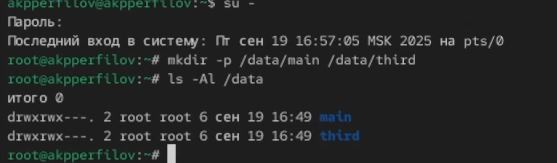
\includegraphics[keepaspectratio]{image/5363977445180569461.jpg}}

}

\caption{Создание каталогов с root}

\end{figure}%

Посмотрим, кто является владельцем этих каталогов. Для этого используем:
ls -Al /data

\begin{figure}[H]

{\centering \pandocbounded{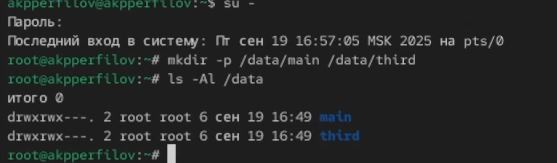
\includegraphics[keepaspectratio]{image/5363977445180569461.jpg}}

}

\caption{Просмотр информации о каталогах}

\end{figure}%

Прежде чем устанавливать разрешения, изменим владельцев этих каталогов с
root на main и third соответственно:

chgrp main /data/main chgrp third /data/third

\begin{figure}[H]

{\centering \pandocbounded{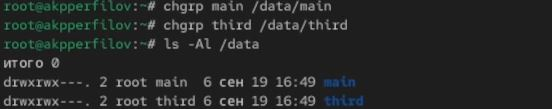
\includegraphics[keepaspectratio]{image/5363977445180569462.jpg}}

}

\caption{Изменение владельцев каталогов}

\end{figure}%

Посмотрим, кто теперь является владельцем этих каталогов: ls -Al /data

\begin{figure}[H]

{\centering \pandocbounded{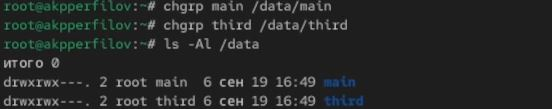
\includegraphics[keepaspectratio]{image/5363977445180569462.jpg}}

}

\caption{Просмотр информации о каталогах}

\end{figure}%

Установим разрешения, позволяющие владельцам каталогов записывать файлы
в эти каталоги и запрещающие доступ к содержимому каталогов всем другим
пользователям и группам:

chmod 770 /data/main chmod 770 /data/third

Проверим установленные права доступа

\begin{figure}[H]

{\centering \pandocbounded{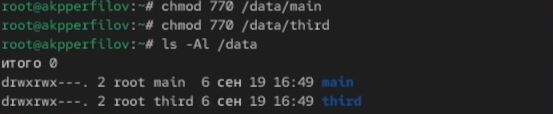
\includegraphics[keepaspectratio]{image/5363977445180569464.jpg}}

}

\caption{Изменение разрешений и просмотр прав доступа}

\end{figure}%

В другом терминале перейдем под учётную запись пользователя bob
Попробуем перейти в каталог /data/main и создать файл emptyfile в этом
каталоге:

cd /data/main touch emptyfile ls -Al

Создался файл с правами под учетную запись пользователя bob

\begin{figure}[H]

{\centering \pandocbounded{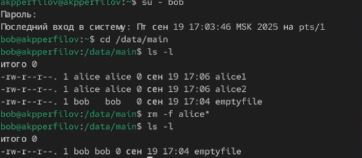
\includegraphics[keepaspectratio]{image/5363977445180569474.jpg}}

}

\caption{Создание файла под учётной записью bob}

\end{figure}%

Под пользователем bob попробуем перейти в каталог /data/third и создать
файл emptyfile в этом каталоге

\begin{figure}[H]

{\centering \pandocbounded{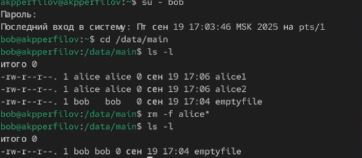
\includegraphics[keepaspectratio]{image/5363977445180569474.jpg}}

}

\caption{Попытка перейти в каталог}

\end{figure}%

\section{Управление специальными
разрешениями}\label{ux443ux43fux440ux430ux432ux43bux435ux43dux438ux435-ux441ux43fux435ux446ux438ux430ux43bux44cux43dux44bux43cux438-ux440ux430ux437ux440ux435ux448ux435ux43dux438ux44fux43cux438}

Откроем новый терминал под пользователем alice. Перейдем в каталог
/data/main: cd /data/main Создадим два файла, владельцем которых
является alice:

touch alice1 touch alice2

\begin{figure}[H]

{\centering \pandocbounded{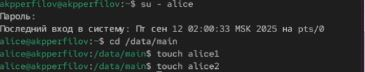
\includegraphics[keepaspectratio]{image/5363977445180569473.jpg}}

}

\caption{Создание файлов под учётной записью alice в каталоге
/data/main}

\end{figure}%

В другом терминале перейдем под учётную запись пользователя bob Перейдем
в каталог /data/main и введем: ls -l

\begin{figure}[H]

{\centering \pandocbounded{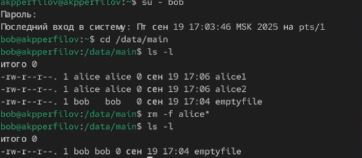
\includegraphics[keepaspectratio]{image/5363977445180569474.jpg}}

}

\caption{Просмотр информации о каталоге}

\end{figure}%

Мы увидим два файла, созданные пользователем alice. Попробуем удалить
файлы, принадлежащие пользователю alice: rm -f alice* Убедимся, что
файлы будут удалены пользователем bob.

\begin{figure}[H]

{\centering \pandocbounded{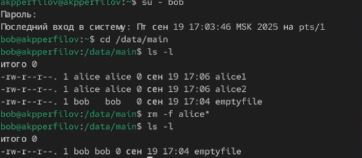
\includegraphics[keepaspectratio]{image/5363977445180569474.jpg}}

}

\caption{Удаление файлов alice и просмотр информации каталога}

\end{figure}%

Создадим два файла, которые принадлежат пользователю bob:

touch bob1 touch bob2

\begin{figure}[H]

{\centering \pandocbounded{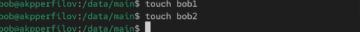
\includegraphics[keepaspectratio]{image/5363977445180569472.jpg}}

}

\caption{Создание файлов под учётной записью bob}

\end{figure}%

В терминале под пользователем root установим для каталога /data/main бит
идентификатора группы, а также stiky-бит для разделяемого (общего)
каталога группы: chmod g+s,o+t /data/main

\begin{figure}[H]

{\centering \pandocbounded{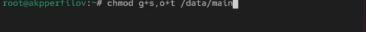
\includegraphics[keepaspectratio]{image/5363977445180569476.jpg}}

}

\caption{Изменение бит индентификатора группы и sticky-бит для общего
каталога группы}

\end{figure}%

В терминале под пользователем alice создадим в каталоге /data/main файлы
alice3 и alice4:

touch alice3 touch alice4 ls -l

Теперь мы должны увидеть, что два созданных нами файла принадлежат
группе main, которая является группой-владельцем каталога /data/main.

\begin{figure}[H]

{\centering \pandocbounded{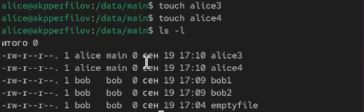
\includegraphics[keepaspectratio]{image/5363977445180569478.jpg}}

}

\caption{Создание файлов и просмотр информации о них}

\end{figure}%

В терминале под пользователем alice попробуем удалить файлы,
принадлежащие пользователю bob: rm -rf bob*

\begin{figure}[H]

{\centering \pandocbounded{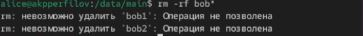
\includegraphics[keepaspectratio]{image/5363977445180569465.jpg}}

}

\caption{Попытка удаление файлов}

\end{figure}%

Как мы видим sticky-bit предотвратил удаление этих файлов пользователем
alice, поскольку этот пользователь не является владельцем этих файлов.
Обратим внимание: поскольку пользователь alice является владельцем
каталога /data/main, то он может удалить все свои файлы в любом случае.

\section{Управление расширенными разрешениями с использованием списков
ACL}\label{ux443ux43fux440ux430ux432ux43bux435ux43dux438ux435-ux440ux430ux441ux448ux438ux440ux435ux43dux43dux44bux43cux438-ux440ux430ux437ux440ux435ux448ux435ux43dux438ux44fux43cux438-ux441-ux438ux441ux43fux43eux43bux44cux437ux43eux432ux430ux43dux438ux435ux43c-ux441ux43fux438ux441ux43aux43eux432-acl}

Применим команды setfacl и getfacl для выполнения поставленной задачи.
Откроем терминал с учётной записью root Установим права на чтение и
выполнение в каталоге /data/main для группы third и права на чтение и
выполнение для группы main в каталоге /data/third:

setfacl -m g:third:rx /data/main setfacl -m g:main:rx /data/third

\begin{figure}[H]

{\centering \pandocbounded{
\includegraphics[keepaspectratio]{image/5363977445180569469.jpg}}

}

\caption{Изменение прав каталогов для групп}

\end{figure}%

Используем команду getfacl, чтобы убедиться в правильности установки
разрешений:

getfacl /data/main getfacl /data/third

\pandocbounded{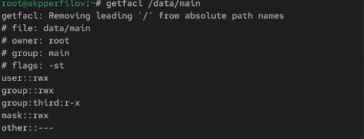
\includegraphics[keepaspectratio]{image/5363977445180569475.jpg}}(image/5363977445180569467.jpg)

Создадим новый файл с именем newfile1 в каталоге /data/main: touch
/data/main/newfile1 Используем getfacl /data/main/newfile1 для проверки
текущих назначений полномочий.

\begin{figure}[H]

{\centering \pandocbounded{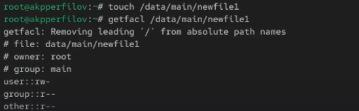
\includegraphics[keepaspectratio]{image/5363977445180569468.jpg}}

}

\caption{Создание файла и просмотр информации о нём}

\end{figure}%

Установим ACL по умолчанию для каталога /data/main: setfacl -m
d:g:third:rwx /data/main

Убедимся, что настройки ACL работают, добавив новый файл в каталог
/data/main: touch /data/main/newfile2

Используем getfacl /data/main/newfile2 для проверки текущих назначений
полномочий

\begin{figure}[H]

{\centering \pandocbounded{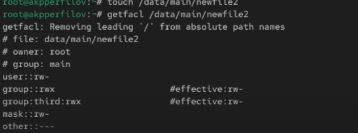
\includegraphics[keepaspectratio]{image/5363977445180569471.jpg}}

}

\caption{Создание файла и просмотр информации}

\end{figure}%

Выполним аналогичные действия для каталога /data/third. Создадим новый
файл newfile2 в каталог /data/third и проверим текущие назначения
полномочий

\begin{figure}[H]

{\centering \pandocbounded{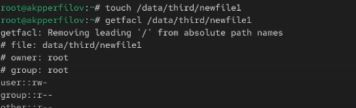
\includegraphics[keepaspectratio]{image/Вставленное изображение.png}}

}

\caption{Создание файла и просмотр информации}

\end{figure}%

Для проверки полномочий группы third в каталоге /data/third войдем в
другом терминале под учётной записью члена группы third: su - carol
Проверим операции с файлами:

rm /data/main/newfile1 rm /data/main/newfile2

\begin{figure}[H]

{\centering \pandocbounded{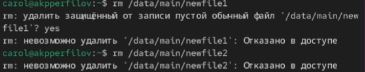
\includegraphics[keepaspectratio]{image/5363977445180569477.jpg}}

}

\caption{Попытка удаление файлов под учётной записью carol}

\end{figure}%

Удалить файлы мы не смогли, так как newfile1 принадлежит пользователю
root и группе main, newfile2 также принадлежит root, main и third, хоть
и carol находится в последней группе, у группы недостаточно прав.

Проверим, возможно ли осуществить запись в файл:

echo \enquote{Hello, world} \textgreater\textgreater{}
/data/main/newfile1 echo \enquote{Hello, world}
\textgreater\textgreater{} /data/main/newfile2

\begin{figure}[H]

{\centering \pandocbounded{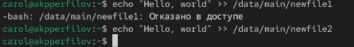
\includegraphics[keepaspectratio]{image/5363977445180569470.jpg}}

}

\caption{Попытка осуществить запись в файлы под учётной записью carol}

\end{figure}%

Мы не смогли осуществить запись в newfile1, так как прав у группы third
на нее нет. А вот уже в newfile2 все получилось, так как права на
изменение файла у данной группы есть.

\chapter{Выводы}\label{ux432ux44bux432ux43eux434ux44b}

Приобретены умения по управлению базовыми и специальными правами доступа
для групп пользователей в ОС Linux.

\chapter*{Список
литературы}\label{ux441ux43fux438ux441ux43eux43a-ux43bux438ux442ux435ux440ux430ux442ux443ux440ux44b}
\addcontentsline{toc}{chapter}{Список литературы}

\printbibliography[heading=none]





\end{document}
